% Si tu trabajo incluye anexos, puedes descomentar las siguientes líneas
\chapter{Annexes}
\label{chap:6_annexes}
\pagenumbering{gobble} % Las páginas de los anexos no se numeran



\section{Optimization results for all the models}
\label{annex:opt_results}

This annex shows the optimization results using TensorRT for all the neural network models used and tested on this work. The inference time results have been stored in several spreadsheets, classified according to the optimization parameters (described in Section \ref{sec:3_swarch}), and a color scale has been added according to the FPS (\textit{Frames per Second}) the resulting graph is capable to process. These numbers are compared as well to the original implementation (GPU without using TensorRT) and to the CPU implementation. The results can be observed in the following subsections.

\subsection{Object detection models}

The optimized models correspond to the different implementations of SSD-based and YOLO-based object detectors, as described in Chapter \ref{chap:2_sota}.

\begin{figure}[h!]
	\centering
	\begin{subfigure}[h]{0.45\linewidth}
		\centering
		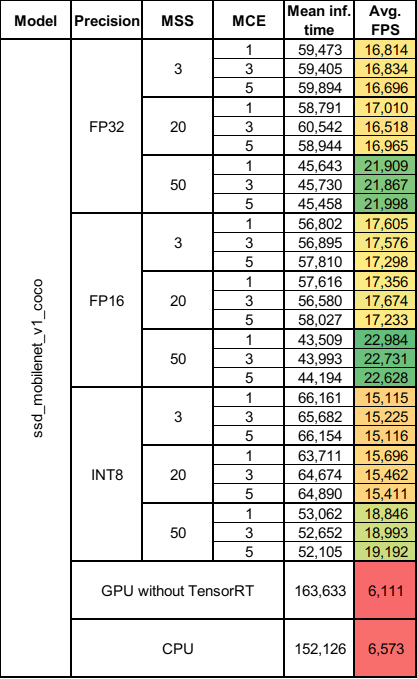
\includegraphics[width=\linewidth]{optimizations_ssd_mobilenet_v1_coco}
		\caption{Optimization results for the object detection model \texttt{ssd\_mobilenet\_v1\_coco}.}
	\end{subfigure}
	\hfill
	\begin{subfigure}[h]{0.45\linewidth}
		\centering
		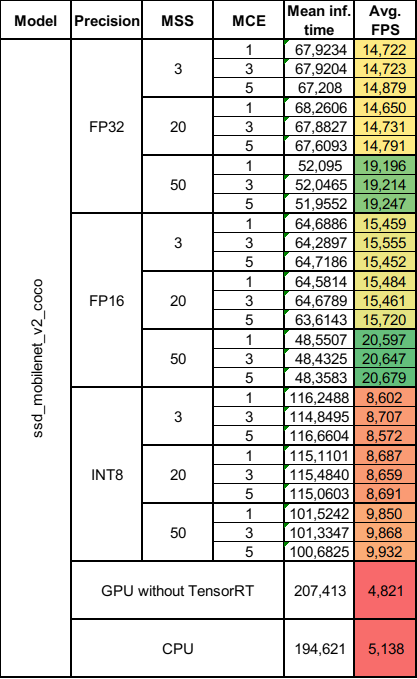
\includegraphics[width=\linewidth]{optimizations_ssd_mobilenet_v2_coco}
		\caption{Optimization results for the object detection model \texttt{ssd\_mobilenet\_v2\_coco}.}
	\end{subfigure}
	\begin{subfigure}[h]{0.45\linewidth}
		\centering
		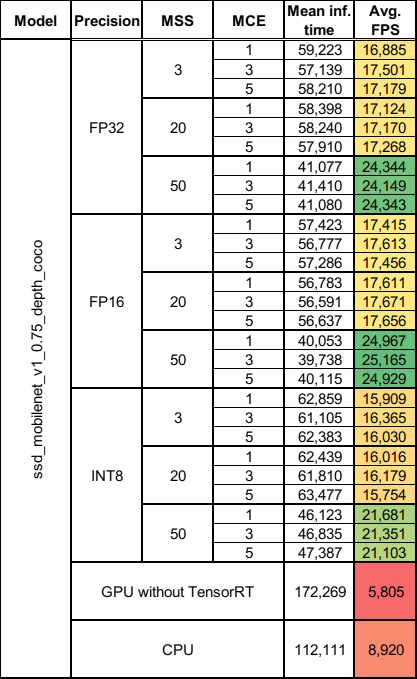
\includegraphics[width=\linewidth]{optimizations_ssd_mobilenet_v1_0.75_depth_coco}
		\caption{Optimization results for the object detection model \texttt{ssd\_mobilenet\_v1\_0\.75\_depth\_coco}.}
	\end{subfigure}
	\hfill
	\begin{subfigure}[h]{0.45\linewidth}
		\centering
		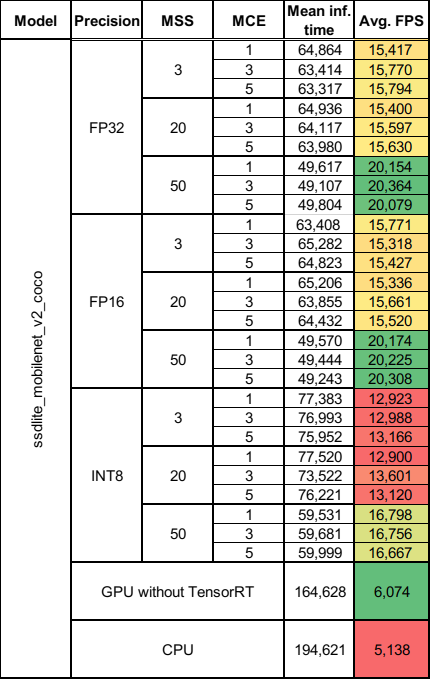
\includegraphics[width=\linewidth]{optimizations_ssdlite_mobilenet_v2_coco}
		\caption{Optimization results for the object detection model \texttt{ssdlite\_mobilenet\_v2\_coco}.}
	\end{subfigure}
	\caption{Optimization results for the SSD-based object detection networks.}
\end{figure}


\begin{figure}[h!]
	\centering
	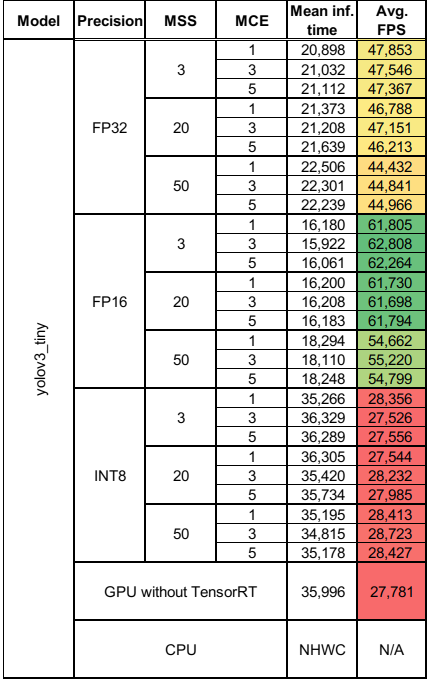
\includegraphics[width=0.45\linewidth]{optimizations_yolov3_tiny}
	\caption{Optimization results for the object detection model \texttt{yolov3\_tiny} (due to hardware compatibility issues, the CPU testing was impossible to perform).}
\end{figure}
\goodbreak
\subsection{Face detection models}

These models are the specifically trained for the \texttt{faced} library \cite{faced}. They have been optimized as well, swapping the originally included models in the package for the TensorRT optimized ones.


\begin{figure}[h!]
	\centering
	\begin{subfigure}[h]{0.45\linewidth}
		\centering
		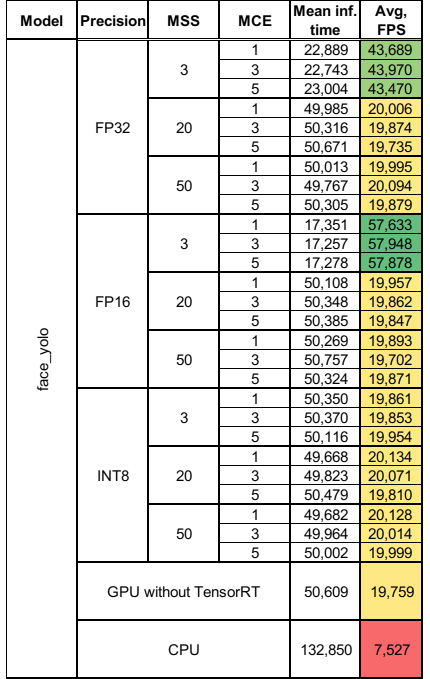
\includegraphics[width=\linewidth]{optimizations_face_yolo}
		\caption{Optimization results for the face detector model \texttt{face\_yolo}.}
	\end{subfigure}
	\hfill
	\begin{subfigure}[h]{0.45\linewidth}
		\centering
		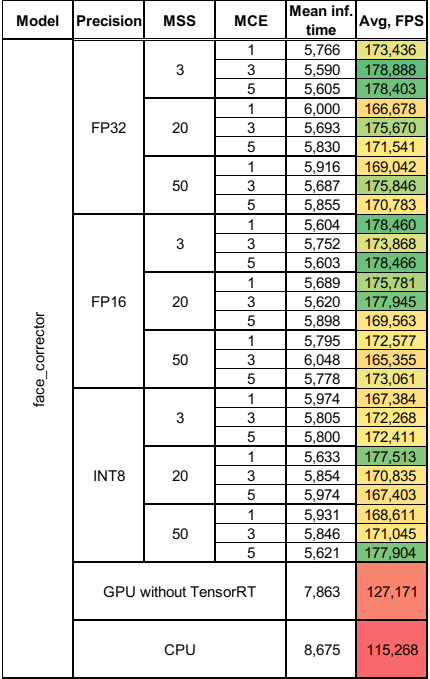
\includegraphics[width=\linewidth]{optimizations_face_corrector}
		\caption{Optimization results for the face corrector mdoel \texttt{face\_corrector}.}
	\end{subfigure}
	\caption{Optimization results for the face detection (\texttt{faced}) networks.}
\end{figure}




\subsection{Face encoding model}
This is the FaceNet implementation \cite{facenet}, which has been optimized as well using TensorRT:

\begin{figure}[h]
	\centering
	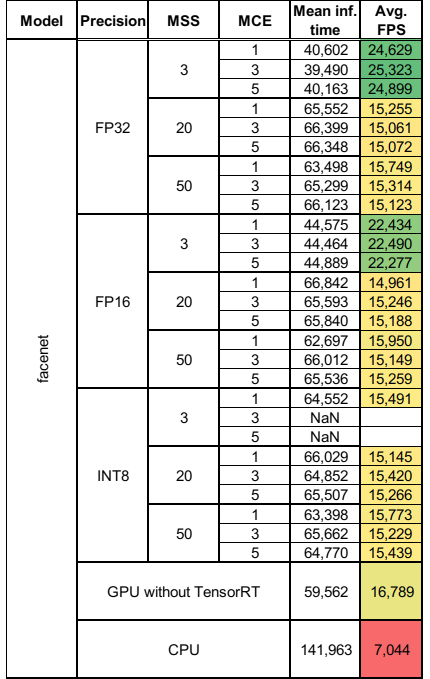
\includegraphics[width=0.5\linewidth]{optimizations_facenet}
	\caption{Optimization results for the face encoding model \texttt{facenet}.}
\end{figure}